% easychair.tex,v 3.5 2017/03/15

\documentclass{easychair}
%\documentclass[EPiC]{easychair}
%\documentclass[EPiCempty]{easychair}
%\documentclass[debug]{easychair}
%\documentclass[verbose]{easychair}
%\documentclass[notimes]{easychair}
%\documentclass[withtimes]{easychair}
%\documentclass[a4paper]{easychair}
%\documentclass[letterpaper]{easychair}

\usepackage{doc}
%\usepackage{amsmath}

% use this if you have a long article and want to create an index
% \usepackage{makeidx}

% In order to save space or manage large tables or figures in a
% landcape-like text, you can use the rotating and pdflscape
% packages. Uncomment the desired from the below.
%
% \usepackage{rotating}
% \usepackage{pdflscape}

% Some of our commands for this guide.
%
\newcommand{\CBCTT}{CB-CTT}
\newcommand{\UP}{UP}
\newcommand{\ASP}{ASP}
\newcommand{\clingo}{\textit{clingo}}
\newcommand{\naf}{\textit{not }} 
\newcommand{\head}{\textit{head}}
\newcommand{\body}{\textit{body}}

%\makeindex

%% Front Matter
%%
% Regular title as in the article class.
%
\title{AI-Based Tool for Curriculum-Based Course Timetabling at the University of Potsdam}

% Authors are joined by \and. Their affiliations are given by \inst, which indexes
% into the list defined using \institute
%
\author{
Christian Dohrmann 
\and
Ulrike Lucke 
\and
Torsten Schaub 
\and 
Sebastian Schellhorn 
}

% Institutes for affiliations are also joined by \and,
\institute{
  University of Potsdam,
  Germany\\
  \email{\{christian.dohrmann, ulrike.lucke, torsten.schaub, sebastian.schellhorn\}@uni-potsdam.de}
 }

%  \authorrunning{} has to be set for the shorter version of the authors' names;
% otherwise a warning will be rendered in the running heads. When processed by
% EasyChair, this command is mandatory: a document without \authorrunning
% will be rejected by EasyChair

\authorrunning{Dohrmann et al.}

% \titlerunning{} has to be set to either the main title or its shorter
% version for the running heads. When processed by
% EasyChair, this command is mandatory: a document without \titlerunning
% will be rejected by EasyChair
\titlerunning{AI-Based Tool for \CBCTT{} of \UP{}}

\begin{document}

\maketitle

\begin{abstract}
  %\begin{itemize}%
    %\item%
    Education is a fundamental component of universities and is linked with the non-trivial possibly time-consuming task of creating suitable timetables for teaching. 
    %\item%
    The corresponding problem is known as Curriculum-Based Course Timetabling, which takes into account various constraints while seeking a conflict-free timetable. %\\
    %\item% 
    We addressed this problem by following a knowledge representation and reasoning approach, describing constraints and feasible assignments of courses to time slots. 
    %\item% 
    Possible assignments are gathered through a prototypical web interface, and the corresponding constraints are respected by automatically finding a timetable using an AI. %\\
    %\item%  
    We discuss the resolved redundancies, time saved and potential future benefits when comparing the traditional and new approach regarding the needs of teachers, students and administration at the University of Potsdam. 
  %\end{itemize}%
\end{abstract}

% The table of contents below is added for your convenience. Please do not use
% the table of contents if you are preparing your paper for publication in the
% EPiC Series or Kalpa Publications series

%\setcounter{tocdepth}{2}
%{\small
%\tableofcontents}

%\section{To mention}
%
%Processing in EasyChair - number of pages.
%
%Examples of how EasyChair processes papers. Caveats (replacement of EC
%class, errors).

%------------------------------------------------------------------------------
\section{Motivation}
\label{sec:motivation}

%\begin{itemize}%
  %\item% 
  Education is a fundamental component of universities, usually addressed by offering a variety of courses that may include lectures, exercises, seminars, projects, etc., within defined study programs. 
  %\item% 
  In order to obtain optimal timetables, all offered courses must be assigned to a time slot and room, while respecting some hard and soft constraints. 
  %\item%
  A time slot is a combination of a day and a time. \\
  %\item%
  The associated problem is known as Curriculum-Based Course Timetabling (\CBCTT{}; \cite{becaroto15}), which takes into account various constraints when seeking a conflict-free timetable. 
  %\item%
  A solution to a \CBCTT{} problem is an assignment of courses to time slots and rooms, such that each corresponding hard constraint is satisfied. 
  %\item%
  For instance, there should be no more than one course assigned to a room and time slot, except when explicitly stated.
  %\item% 
  An optimal solution is a solution with minimal penalties regarding soft constraints. \\
  %\item% 
  Traditionally, solving \CBCTT{} problems involve human efforts, consuming a significant amount of time and requiring numerous agreements.
  %\item% 
  Especially when multiple individuals are involved in developing timetables, redundancies and conflicts among the resulting plans may arise.
  %\item% 
  In addition, the obtained timetables are often not guaranteed to be optimal and may possibly violate soft or hard constraints. \\
  %\item% 
  In our work, we model the relevant soft and hard constraints within the context of the University of Potsdam (\UP{}) to obtain conflict-free and optimal timetables derived by an AI. 
  %\item%
  Thanks to its simple modeling language and high-performance solving capabilities, Answer Set Programming (\ASP{}; \cite{baral02a}) is a well-suited approach for knowledge representation and reasoning in modeling \CBCTT{} problems, as demonstrated by \cite{bainkaokscsotawa18a}.
  %\item% 
  We developed a prototypical web interface allowing planners and lecturers to enter availabilities for teaching times and suitable rooms regarding courses. 
  %\item% 
  This interface can automatically generate a timetable within seconds, ensuring compliance with the required constraints among curricula across all  involved institutes and planners. 
  %\item%
  The idea is to find a solution from the time slots specified by lecturers rather than permitting any course to potentially take place at any time slot.
  %\item%
  As a goal, the obtained timetables should automatically result into corresponding room reservations at universities course catalog. \\
  %\item%
  The remaining article first compares the traditional and new appraoch of solving \CBCTT{} problems at the \UP{} in Section~\ref{sec:approach}. 
  %\item%
  In Section~\ref{sec:asp}, we introduce basics of our knowledge representation and reasoning approach and illustrate modeled constraints. 
  %\item%
  Afterwards, in Sections~\ref{sec:impact} and \ref{sec:future}, we sketch resolved redundancies, time savings and possible future benefits.
%\end{itemize}%


%------------------------------------------------------------------------------
\section{Overall Approach}
\label{sec:approach}

%\begin{itemize}% 
  %\item% 
  In the following, we describe the traditional and new approach of finding a timetable and link it to the course catalog at \UP{}. 
  %\item% 
  To this end, let us first describe the structure and relationships among curricula, modules, examination tasks and courses. \\
  %\item%
  A cohort of students is given by a corresponding program and semester wrt the curriculum. 
  %\item% 
  Each curriculum is defined by referring to modules needed to be accomplished. 
  %\item% 
  Modules specify the number and type of courses and course components, along with their primary and secondary examination tasks. 
  %\item%
  For simplicity, in the following, we use the term \textit{courses} to refer to both courses and course components, explicitly indicating the distinction when necessary. 
  %\item% 
  Courses are linked to, possibly several, secondary and sometimes primary examination tasks within a set of modules. 
  %\item%  
  As modules are associated with possibly several curricula, the linkage of examination tasks to courses induces involved curricula and cohorts possibly participate to a course. 
  %\item% 
  Whenever a module occurs in several curricula, possibly of different institutes or faculties, then the objective to find a conflict-free timetable becomes more complicated. \\
  %\item% 
  In the traditional case, lectures with a large number of participants are planned first, due to a limited number of large lecture halls and imports/exports of courses among curricula. 
  %\item% 
  The resulting timetable regarding large lectures needs a lot of communication and agreements among several planners to ensure a conflict-free timetable for involved cohorts and lecturers. 
  %\item% 
  Especially, in the case of degree programmes that aim to train teachers with allowed combinations of subjects, \UP{} has developed a so called time frame model to prevent conflicts among courses of most common combinations of topics\footnote{https://www.uni-potsdam.de/en/studium/studying/organizing-your-studies/potsdams-time-frame-model}.
  %\item% 
  On top of scheduled large lectures, the remaining courses are planned by the respective planners of each institute to achieve suitable timetables. 
  %\item% 
  A timetable should avoid conflicts regarding multiple use of rooms, lecturers and cohorts as well as respecting particular demands of courses, like technical equipment.
  %\item% 
  A timetable is considered more optimal, if it respects for instance traveling time of consecutive courses, teaching load per day and gaps among courses of a day aiming on same cohort or lecturer, respectively. 
  %\item% 
  Once a solution is found, each planner must manually copy it, course by course, to the universities course catalog, link each course to examination tasks of particular modules and book a room for the assigned time slot. \\
  %\item% 
  Our approach aims to minimize time-consuming communication among planners and lecturers, as well as reduce redundancies when a solution is found but needs to be copied to the course catalog, linked to modules, and booked into rooms.
  %\item% 
  To this end, we developed a prototypical web interface that enables planners and lecturers to collaboratively create courses and course components, providing all necessary information to facilitate finding a feasible solution.
  %\item%
  In more detail, for each course, the system requests a name, a list of linked modules, specification of whether it is offered in the winter or summer term, and the designation of a responsible planner.
  %\item% 
  The web interface allows to state the type, e.g. lecture or seminar, the expected number of participants and any specific equipment requirements, e.g. large board, for each course component.  
  %\item%
  Furthermore, for each course component, particular rooms, days and times, along with a priority can be selected.
  %\item% 
  Through  the cross product of days, times and rooms possible prioritized availabilities are established for each course component. 
  %\item% 
  See figure~\ref{fig:web interface} illustrating parts of the prototypical web interface. 
  \begin{figure}
    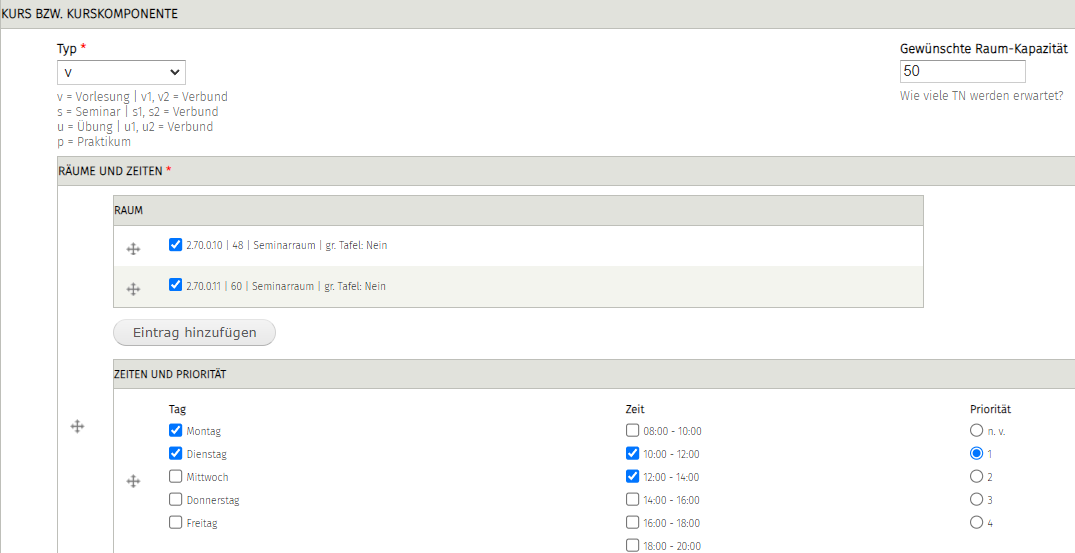
\includegraphics[width=\linewidth]{webinterface}
    \caption{Web interface inducing 18 availabilities of highest priority 1 and three availabilities of priority 2 for a seminar with expected number of 30 participants.}
    \label{fig:web interface}
  \end{figure}
  %\item% 
  We identified and provided four pairwise relations to capture significant constraints among course components: \newpage
  \begin{itemize}
    \item Two course components are not allowed to take place in parallel, e.g. obligatory lectures for the same cohort.
    \item Two course components have to take place in parallel (same time slot, but different rooms), e.g. two groups of exercises for the same course.
    \item Two course components have to take place simultaneous (same time slot and room), e.g. hosting two seminars, with different names but sharing major content, in the same room.
    \item Two course components have to take place consecutive, e.g. having an exercise directly after the corresponding lecture. 
  \end{itemize}
  %\item%
  These four relations allow us to pose certain structures among course components, which enable or disable underlying constraints as elaborated in the next section. \\ 
  %\item%
  The corresponding planner verifies the consistency and correctness of the input data for the web interface. 
  %\item% 
  The input data, along with a logic representation of necessary constraints, is given to an AI problem solver, which then searches for an optimal timetable. 
  %\item%
  Intuitively, the data collected by the web interface can be understood as a particular problem instance and the logic representation of constraints can be understood as a general and persistent problem description. 
  %\item%
  The output is a visualization of the resulting timetable and is double-checked by planners. 
  %\item%
  As an example of a resulting timetable see figure~\ref{fig:timetable}. 
  \begin{figure}
    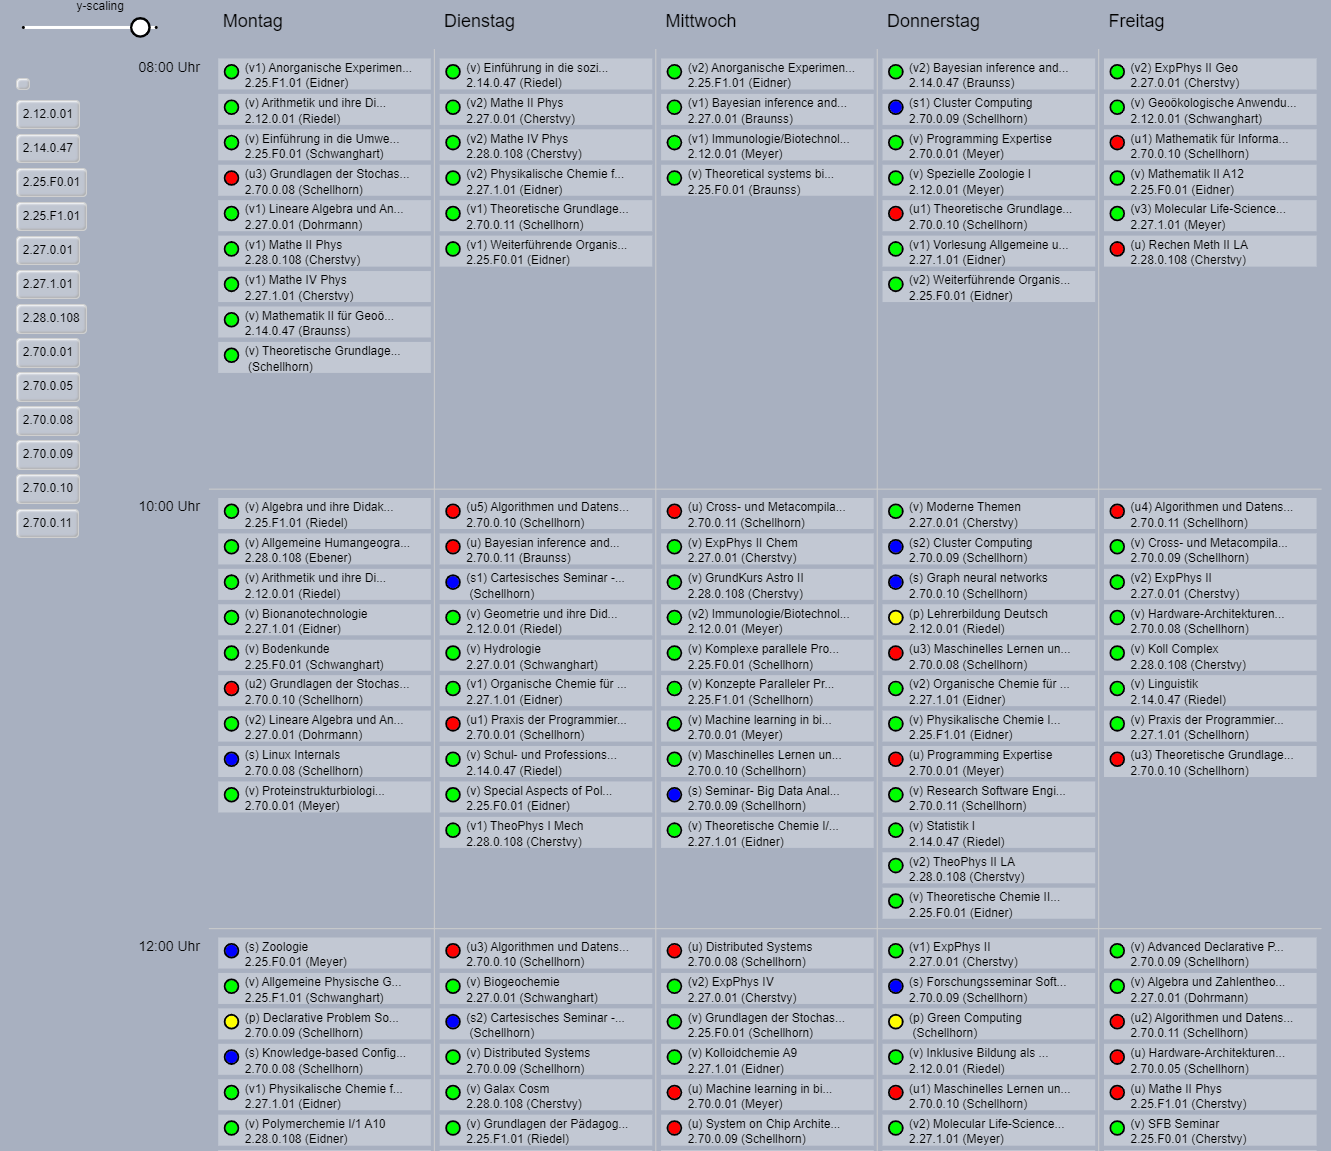
\includegraphics[width=\linewidth]{timetable}
    \caption{Part of the resulting timetable containing about 200 course components at the Faculty of Science for summer term 2024.}
    \label{fig:timetable}
  \end{figure} \\
  %\item% 
  Note that the new approach aligns with the traditional idea of splitting the process into two steps: initially finding a timetable for large lectures and subsequently completing it to a timetable for each institute.
  %\item% 
  The resulting timetable for each institute must be (automatically) transferred to the university's course catalog, taking into account linked modules, lecturers, time slots, and rooms.
  %\item% 
  The final step of automatically integrating the obtained timetable into the course catalog is not yet implemented in the prototype but will eventually eliminate many redundancies.
%\end{itemize}%


%------------------------------------------------------------------------------
\section{Technical Solution: \ASP{} Paradigm}
\label{sec:asp}
%\begin{itemize}%
  %\item% 
  \ASP{} \cite{baral02a, breitr11a} is an approach to declarative problem solving and belongs to the area of knowledge representation and reasoning. 
  %\item% 
  The roots of \ASP{} go back to logic programming, nonmonotonic reasoning and constraint satisfaction \cite{gellif91a}. 
  %\item% 
  The idea of \ASP{} is to describe the problem using a formal representation, rather than instructing a computer how to solve the problem. 
  %\item% 
  Figure~\ref{fig:asp} illustrates this approach \cite{gekakasc12a}. 
  \begin{figure}
  \label{fig:asp}
  \begin{center}{%
    \begin{picture}(300,120)(-150,-60)
    \put(-80,+40){\makebox(0,0){\framebox(80,20){Problem}}}
    \put(-80,-40){\makebox(0,0){\framebox(80,20){Logic Program}}}
    \put(+80,+40){\makebox(0,0){\framebox(80,20){Solution}}}
    \put(+80,-40){\makebox(0,0){\framebox(80,20){Stable Models}}}
    \put(-80,+30){\vector(0,-1){60}}
    \put(-40,-40){\vector(+1,0){80}}
    \put(+80,-30){\vector(0,+1){60}}
    \put(-110,  0){\makebox(0,0){Modeling}}
    \put(+120,  0){\makebox(0,0){Interpreting}}
    \put(   0,-55){\makebox(0,0){{Solving}}}
    \end{picture}}
    \end{center}
  \caption{Schematic representation of declarative problem solving process.}
  \end{figure} \\
  %\item% 
  An easy and human-readable modeling language \cite{cafageiakakrlemarisc19a} is used to create a logic program modeling the original problem. 
  %\item%
  By utilizing a problem solver such as \clingo{} \cite{gekakaosscwa16a}, a solution, i.e. a stable model \cite{gellif88b}, of the problem is found and has to be interpreted by the user. 
  %\item% 
  Due to its simple but rich high-level modeling language, its elaboration-tolerance, and its high-performance solving capacities, \ASP{} becomes a well suited approach to model real-world problems. \\
  %\item% 
  The range of applications for modeling and solving combinatorial search problems with \ASP{} spans across various domains, including planning, scheduling, configuration, probabilistic reasoning, diagnosis and repair, classification, query answering, explanation generation, multi-agent systems, natural language processing, computational biology, music composition, model checking and robotics \cite{ergele16}. 
  %\item% 
  In Terms of industrial applications, \ASP{} has been successfully employed for solving (automated product) configuration \cite{soinie99a, hebasasc22a}, planning \cite{jizhkhst19a, sopobasc23a}, scheduling \cite{aldoma17a}, timetabling \cite{bainkaokscsotawa18a} and other problems \cite{fafrsctate18a}. 
  %\item%
  Especially for industrial applications, tackled by a declarative approach like \ASP{}, significant improvements wrt implementation, maintenance costs and human-machine interaction were shown. 
  %\item% 
  For instance, Siemens reported saving more than 80\% of maintenance costs by using a knowledge representation and reasoning approach, as mentioned in \cite{fafrhascsc16a}. 
%\end{itemize}%

\subsection{Modeling with \ASP{}}
\label{subsec:asp}
%\begin{itemize}%
  %\item%
  \ASP{} provides a powerful high-level modeling language that supports recursive definitions, default negation for dealing with the absence of information, disjunctions, aggregates, weight constraints, optimization statements and external atoms. 
  %\item%
  In the following, we provide a brief introduction to the basics of the modeling language of \ASP{} \cite{cafageiakakrlemarisc19a} and the stable models semantics of logic programs \cite{gellif88b}. \\
  %\item% 
  Terms are either constants, variables, arithmetic terms or functional terms. 
  %\item% 
  Constants are denoted by strings starting with lowercase letter, quoted strings or integers. 
  %\item%
  Variables are denoted by strings starting with uppercase letter. 
  %\item% 
  A predicate atom, is of form $p(t_1,\dots,t_n)$, where $p$ is a predicate name, $t_1,\dots,t_n$ are terms and $n\geq0$ is the arity of the predicate atom. 
  %\item% 
  Predicate atoms of arity $0$ are represented by its name without parentheses.
  %\item% 
  In the following, predicate atoms are called atoms for short and are denoted by $a$.
  %\item% 
  An atom is called ground and can be understood as propositional, if all its variables are substituted by constants. 
  %\item%
  A literal is an atom $a$ or its default negation $\naf{} a$. 
  %\item% 
  Default negation, also known as negation as failure, refers to the absence of information, whereas "classical" negation induces the presence of negated information. \\
  %\item% 
  A rule $r$ is of form 
  \begin{align*}
    a_0 \leftarrow a_1,\dots,a_n, \naf{} a_{n+1},\dots,\naf{} a_m
  \end{align*}
  where $0\leq n\leq m$ and each $a_i$ is an atom for $1\leq i \leq m$. 
  %\item% 
  Let $\head{(r)} = a_0$ and $\body{(r)} = \{a_1,\dots,a_n,\naf{} a_{n+1},\dots,\naf{} a_m\}$ the head and the body of a rule $r$, respectively. 
  %\item% 
  For a set of literals $X$, let $X^+ = \{a \mid a\in X \}$ and $X^- = \{a \mid \naf{} a\in X\}$. 
  %\item% 
  Intuitively, the $\head{(r)}$ of a rule $r$ must hold, if the $\body{(r)}$ holds. 
  %\item% 
  The body $\body{(r)}$ of rule $r$ holds, if atoms of $\body{(r)}^+$ are provably true and atoms of $\body{(r)}^-$ are possibly false. 
  %\item% 
  A rule $r$ is called fact, whenever $\body{(r)}=\emptyset$.\footnote{Usually, we drop $\leftarrow$ in this case.} 
  %\item% 
  A rule $r$ is called (integrity) constraint, whenever $\head{(r)}\cap\body{(r)}^-\neq\emptyset$. %\footnote{Usually, literals $\head{(r)}$ and $\naf{} \head{(r)}$ are dropped in this case.}
  %\item% 
  Integrity constraints are used to eliminate unintended solution candidates, whenever its body is satisfied. \\
  %\item% 
  As an example, consider rule 
  \lstinputlisting[basicstyle=\ttfamily\small, firstline=27, lastline=31]{example.lp} %TODO: Listing style von potassco solution 
  deriving a conflict among two course components of ``AI'' lecture and exercise that shall take place consecutive, whenever they are scheduled on a different day than friday.\footnote{In the syntax of an \ASP{} encoding `$\leftarrow$' is represented by `$:-$' and each rule terminates by a period `.'.}  \\
  %\item%
  A logic program is a finite set of rules. 
  %\item% 
  A set of ground atoms $X$ is a model of a logic program $P$, if for every $r\in P$ holds $\head{(r)}\in X$ whenever $\body{(r)}^+\subseteq X$ and $\body{(r)}^-\cap X=\emptyset$.
  %\item% 
  The stable model of a program $P$ is defined relative to a set of atoms $X$, by the so called reduct $P^X$, defined by 
  \begin{align*}
    P^X=\{\head{(r)}\leftarrow \body{(r)}^+\mid r\in P, \body{(r)}^-\cap X = \emptyset\}.
  \end{align*}
  %\item% 
  $X$ is a stable model of a program $P$, if $X$ is the $\subseteq$-minimal model of $P^X$. \\
  %\item% 
  As an example consider the following program $P_1$
  \lstinputlisting[basicstyle=\ttfamily\small, numbers=left]{example.lp}
  where lines 1-21 are facts setting rooms, room capacities, course components with expected number of participants, stating ``AI'' lecture and exercise as consecutive as well as declaring possible time slots and rooms for each course component. 
  %\item% 
  Line 22 sets ``AI'' lecture to time slot with identifier 42, since there is no other option. 
  %\item% 
  Lines 23-26 state that either time slot with identifier 43 or 44 has to be taken for the ``AI'' exercise. 
  %\item% 
  Lines 27-31 derive a conflict predicate, whenever ``AI'' lecture and exercise are not at same day and thus not consecutive. 
  %\item% 
  Lines 32-33 form an integrity constraint ruling out models containing conflict predicate derived by lines 27-31. 
  %\item% 
  Since atoms of lines 1-21 are facts, they belong to any model of $P_1$. 
  %\item% 
  Let $X$ be the set containing atoms of lines 1-21. 
  %\item% 
  Note that $X$ is not a model of $P_1$, since the body of rule in line 22 is satisfied, but not its head. 
  %\item% 
  Sets 
  \begin{align*}
    X\cup&\{\texttt{book(42, ("AI", v)), book(43, ("AI", u)),} \\
         &\texttt{conflict(consecutive, ((42, ("AI", v)), (43, ("AI", u)))), conflict}\}
  \end{align*} 
  and 
  \begin{align*}
    X\cup\{\texttt{book(42, ("AI", v)), book(44, ("AI", u))}\}
  \end{align*} 
  are models of $P_1$, but the latter one is the only stable model of $P_1$, since first model is not $\subseteq$-minimal under reduct wrt $P_1$, due to 
  \begin{align*}
    X\cup&\{\texttt{book(42, ("AI", v)), book(43, ("AI", u)),} \\
         &\texttt{conflict(consecutive, ((42, ("AI", v)), (43, ("AI", u))))}\}.
  \end{align*} \\
  %\item% 
  The basic approach of modeling a problem by an \ASP{} encoding follows a generate-and-test methodology, also known as guess-and-check, inspired by intuitions on \textit{NP} problems. 
  %\item% 
  NP problems are problems, where no algorithm is known to solve them in polynomial time. 
  %\item%
  Intuitively, NP problems are hard to solve, since the needed time may grow exponentially. 
  %\item%  
  In the case of \CBCTT{} for a generate-and-test methodology, one could think of generating any timetable as a model and eliminating certain models by imposing specific (hard) constraints.
%\end{itemize}%

\subsection{Modeling Curriculum-Based Course Timetabling}% at the University of Potsdam}
\label{subsec:modeling}
%\begin{itemize}%
  %\item% 
  Since a course may consists of several course components of possibly different types, e.g. a lecture and an exercise, we identify a course component by a unique tuple of a name and its type, e.g. lecture \textit{(``AI'', v)} and exercise \textit{(``AI'', u)} of the course named Artificial Intelligence. \\
  %\item%
  We modeled the following hard (H0-8) and soft (S0-13) constraints. 

  \textbf{H0.} Components: No component of a course should take place in parallel to its corresponding lecture, except if explicitly stated. 

  \textbf{H1.} Courses: One availability for each course component must be assigned to a time slot and room. 

  \textbf{H2.} Cohort: Obligatory lectures of the same cohort must be all scheduled in different time slots, except explicitly stated to take place in parallel. 

  \textbf{H3.} RoomOccupancy: Two course components cannot take place in the same room and time slot, except explicitly stated. 

  \textbf{H4.} Lecturer: Course components sharing a lecturer cannot be scheduled in parallel, except explicitly stated. 

  \textbf{H5.} NotParallel: Avoiding two course components to take place in parallel, whenever explicitly stated.

  \textbf{H6.} Parallel: Two course components have to take place in parallel, whenever explicitly stated.

  \textbf{H7.} Simultaneous: Two course components have to take place simultaneously, whenever explicitly stated.

  \textbf{H8.} Consecutive: Two course components have to be scheduled consecutively, whenever explicitly stated.

  \textbf{S0.} Availability: For each course component, try to serve prioritized availability on time slot and room. The penalty points reflect corresponding priorities.  

  \textbf{S1.} RoomCapacity: For each course component, penalty points for the number of students that are expected to attend the course minus the number of seats in the corresponding room are imposed on each violation. 

  \textbf{S2.} Cohort: Course components addressed to the same cohort should be scheduled in different time slots, except explicitly stated to be in parallel. Each violation counts as a penalty point. 

  \textbf{S3.} Gaps: For a cohort as well as a lecturer, corresponding course components should be scheduled in time slots as close as possible. The penalty regarding two courses sharing a cohort or lecturer and a day is given by subtracting the earlier time from the later time. 

  \textbf{S4.} RoomStability: Two course components stated to be consecutive should be booked in the same room. The penalty points reflect each violation. 

  \textbf{S5.} MaxLoad: For a cohort as well as lecturer the number of corresponding course components per day should be lower or equal to a given maximum. The penalty points reflect the number of courses beyond the maximum. 

  \textbf{S6.} TravelTime: For a cohort as well as a lecturer, traveling time between rooms with two adjacent course components should be as small as possible. The penalty is reflected by the traveling time itself. 

  \textbf{S7-13.} RoomSuitability: Some course components prefer particular equipment like a large board, projector, computer, microphone, camera, media table or whiteboard. Each violation counts as a penalty point. 

  %\item% 
  Note that some constraints are similar to those presented in \cite{bainkaokscsotawa18a}, others are modified or new.
  %\item% 
  Due to lack of space, we omit the corresponding logic program here.\footnote{The particular \ASP{} encoding representing above constraints can be found at GitHub: https://github.com/schellhorn/CBCTT-UP.} 
  %\item% 
  Optimization aims to minimize penalty points associated with the aforementioned soft constraints. \\
  %\item%
  The system of \cite{bainkaokscsotawa18a} reads instances in a standard input format \cite{bocegasc12a}, translates them into \ASP{} facts and assigns potentially any course to any time slot. 
  %\item%
  In contrast, we employed a direct modeling approach tailored to the constraints and requirements of the \UP{}, which partially is not covered by the standard input format of the \CBCTT{} community. 
  %\item%
  As a design decision, we reduced the search space to collected availabilities only, rather than of checking for all possible time slots and rooms for each course component.
%\end{itemize}%


%------------------------------------------------------------------------------
\section{Results and Impact}
\label{sec:impact}
%\begin{itemize}%
  %\item%
  In \cite{bainkaokscsotawa18a}, it was demonstrated that addressing \CBCTT{} problems through an \ASP{}-based approach outperforms other state-of-the-art approaches and thus makes it well-suited to tackle \CBCTT{} problems. 
  %\item% 
  Our real world approach is still at a prototypical stage and it is lacking (automated) access to some data needed to apply all presented and modeled constraints. \\
  %\item%
  For the winter semester of 2023/24, an optimal and conflict-free plan was found for approximately 160 courses aimed at large lecture halls of the Faculty of Science, additional 90 courses of the Institute of Mathematics and 100 courses of the Institute of Computer Science, incorporating constraints H1, H3, H5, S0, S1 and S7 from the above \ASP{}-based modeling. 
  %\item% 
  Analogously, for the summer semester of 2024, an optimal and conflict-free plan was found involving about 200 courses and constraints H0, H1, H3, H5, H6, H7, H8, S0, S1, S4 and S7.  
  %\item% 
  The \clingo{} solver was integrated into the web interface and required approximately  170 seconds for the winter and less than one second for the summer semester, respectively, to schedule the curricula for the faculty. 
  %\item% 
  Finding plans for each institute took less than a second. 
  %\item%
  The time required to solve these problems relative to the number of involved courses highlights the exponential complexity inherent in \CBCTT{} problems. 
  %\item% 
  For this reason, it is crucial to maintain a workflow that breaks down the planning task into several smaller tasks, similar to the traditional approach. \\
  %\item% 
  A major benefit of the presented AI-based approach is its fairness, transparency and elaboration tolerance. 
  %\item% 
  Thanks to its elaboration tolerance, the existing encoding can be reused for finding a plan for each upcoming semester as it only depends on given courses. 
  %\item% 
  It is possible to add new constraints or relax existing ones whenever needed to address the particular demands of institutes or faculties. 
  %\item% 
  Planners and lecturers can set a prioritized selection of availabilities and preferences for upcoming teaching periods, resulting in an optimal and provably conflict-free timetable.
  %\item% 
  Obtaining a conflict-free timetable for a faculty in a matter of seconds, while respecting dependencies among the several institutes at the same time, resolves a significant amount of communication overhead and conflicts inherent in the traditional approach. 
  %\item% 
  Thus, our approach provides planners with the opportunity to allocate their additional available time to other tasks. \\
  %\item% 
  Once the integration of the resulting timetable into the university's course catalog is done automatically, even more redundancies are resolved, and a considerable amount of additional human capacities become available. 
  %\item% 
  Due to our current prototypical state, we have not yet conducted a performance comparison with other approaches\cite{feutrier23a}. 
%\end{itemize}%


%------------------------------------------------------------------------------
%\section{Related Work} % no time to check for it properly
%\label{sec:related}
%... 


%------------------------------------------------------------------------------
\section{Future Work}
\label{sec:future}
%\begin{itemize}%
  %\item% 
  In future, we plan to implement an interface that allows us to access data such as previous course catalogues, curricula, and their modules.
  %\item% 
  Furthermore, we plan to develop an interface that allows us to automatically push final timetables to the university's course catalog. \\
  %\item% 
  Another non-trivial task is to provide opportunities to the user to analyze and solve conflicts whenever needed.  
  %\item% 
  In a next step, we plan to expand the number of users and involve them in a feedback loop to enhance the usage of the system and identify additional needs.
  %\item% 
  In the long run, one could think about adding functionalities such as drag and drop to manually incorporate smaller changes to a calculated timetable, while preserving consistency regarding hard and soft constraints. \\
  %\item% 
  When establishing the mentioned workflow to obtain conflict-free timetables, one could measure the average amount of time needed per planner using the traditional and new approach, respectively.
  %\item% 
  Moreover, one could compare the quality of resulting timetables regarding the desired hard and soft constraints. 
  %\item% 
  Comparing the quality and time efficiency of both approaches may highlight the usage and impact of our new approach using AI of knowledge representation and reasoning. \\
  %\item% 
  The data about availabilities of different types of course components in various time slots provides insights into the needs of room infrastructure. 
  %\item% 
  One could consider possibly leveraging entered availabilities and the number of participants to derive the location, size, and quantity of needed lecture halls and seminar rooms when planning to build new ones. \\
  %\item% 
  Finally, our approach has significant potential to eliminate redundant workflows, promotes trustworthy collaborations among institutes, save money, and elevate administrative planning tasks to the next level. 
%\end{itemize}% 


\label{sec:bib}
\bibliographystyle{plain}
%\bibliographystyle{alpha}
%\bibliographystyle{unsrt}
%\bibliographystyle{abbrv}
\bibliography{refs} % TODO: consistence eg for first names


%------------------------------------------------------------------------------
% Index
%\printindex

%------------------------------------------------------------------------------
\end{document}

